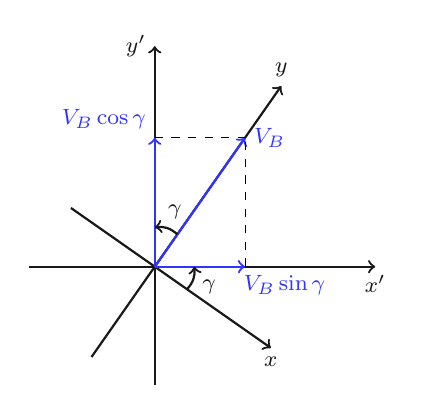
\begin{tikzpicture}
  \begin{scope}
    \footnotesize
    \draw[->,thick,black!90] (-1.6,0) -- (2.8,0) node[below] {$x'$};
    \draw[->,thick,black!90] (0,-1.5) -- (0,2.8) node[left] {$y'$};
    \draw[->,thick,rotate=-35,black!90] (-1.3,0) -- (1.8,0) node[below] {$x$};
    \draw[->,thick,rotate=-35,black!90] (0,-1.4) -- (0,2.8) node[above] {$y$};

    \draw[->,thick,blue!80,rotate=-35] (0,0) -- (0,2) coordinate(Va) node[right] {$V_B$};
    \draw[-,dashed] (0,{2*cos(35)}) -- (Va);
    \draw[->,thick,blue!80] (0,0) -- (0,{2*cos(35)}) node[above left] {$V_B\cos\gamma$};
    \draw[-,dashed] ({2*sin(35)},0) -- (Va);
    \draw[->,thick,blue!80] (0,0) -- ({2*sin(35)},0) node[below,xshift=5mm] {$V_B\sin\gamma$};

    \path[->,thick,black!90] ({.5*sin(35)},{.5*cos(35)}) edge [bend right=25] node[above,xshift=1mm] {$\gamma$} (0,.5);
    \path[->,thick,black!90] ({.5*cos(35)},{-.5*sin(35)}) edge [bend right=25] node[right,yshift=-1mm] {$\gamma$} (.5,0);
  \end{scope}
\end{tikzpicture}